\chapter{复杂CPU设计实现（WIRED）}\label{chap:05-complex-cpu}

\section{Wired 简介}\label{sec:05-complex-cpu-001}

Wired 是一个基于 Loongarch32 完整指令集（包括浮点）的 CPU 核。Wired 核对先进微架构设计及对称多处理器（SMP）设计进行了尝试和探索，成功地实现了乱序双发射且支持硬件缓存一致性的内核微架构。

本核心已验证可以通过 Chiplab（Verilator）进行仿真，并通过 Xilinx Vivado 综合到 FPGA 平台进行验证。

Wired 核心整体基于 Tomasulo 算法的思路实现动态调度，采用基于 ROB 的寄存器重命名策略，并实现了分支预测、数据旁路、推测唤醒等机制以提高流水线效率。 Wired 完整实现了 Loongarch32 指令集中的所有整数指令及绝大部分单精度浮点指令，提供单精度浮点执行支持。 对于部分特殊单精度浮点指令 (frsqrt.s、fmina.s、fmaxa.s) 没有进行相应的实现，而这部分指令也不并会被编译器生成。

核心整体架构如图\ref{fig:05-wired-arch}。

\begin{figure}[htbp]
  \centering
  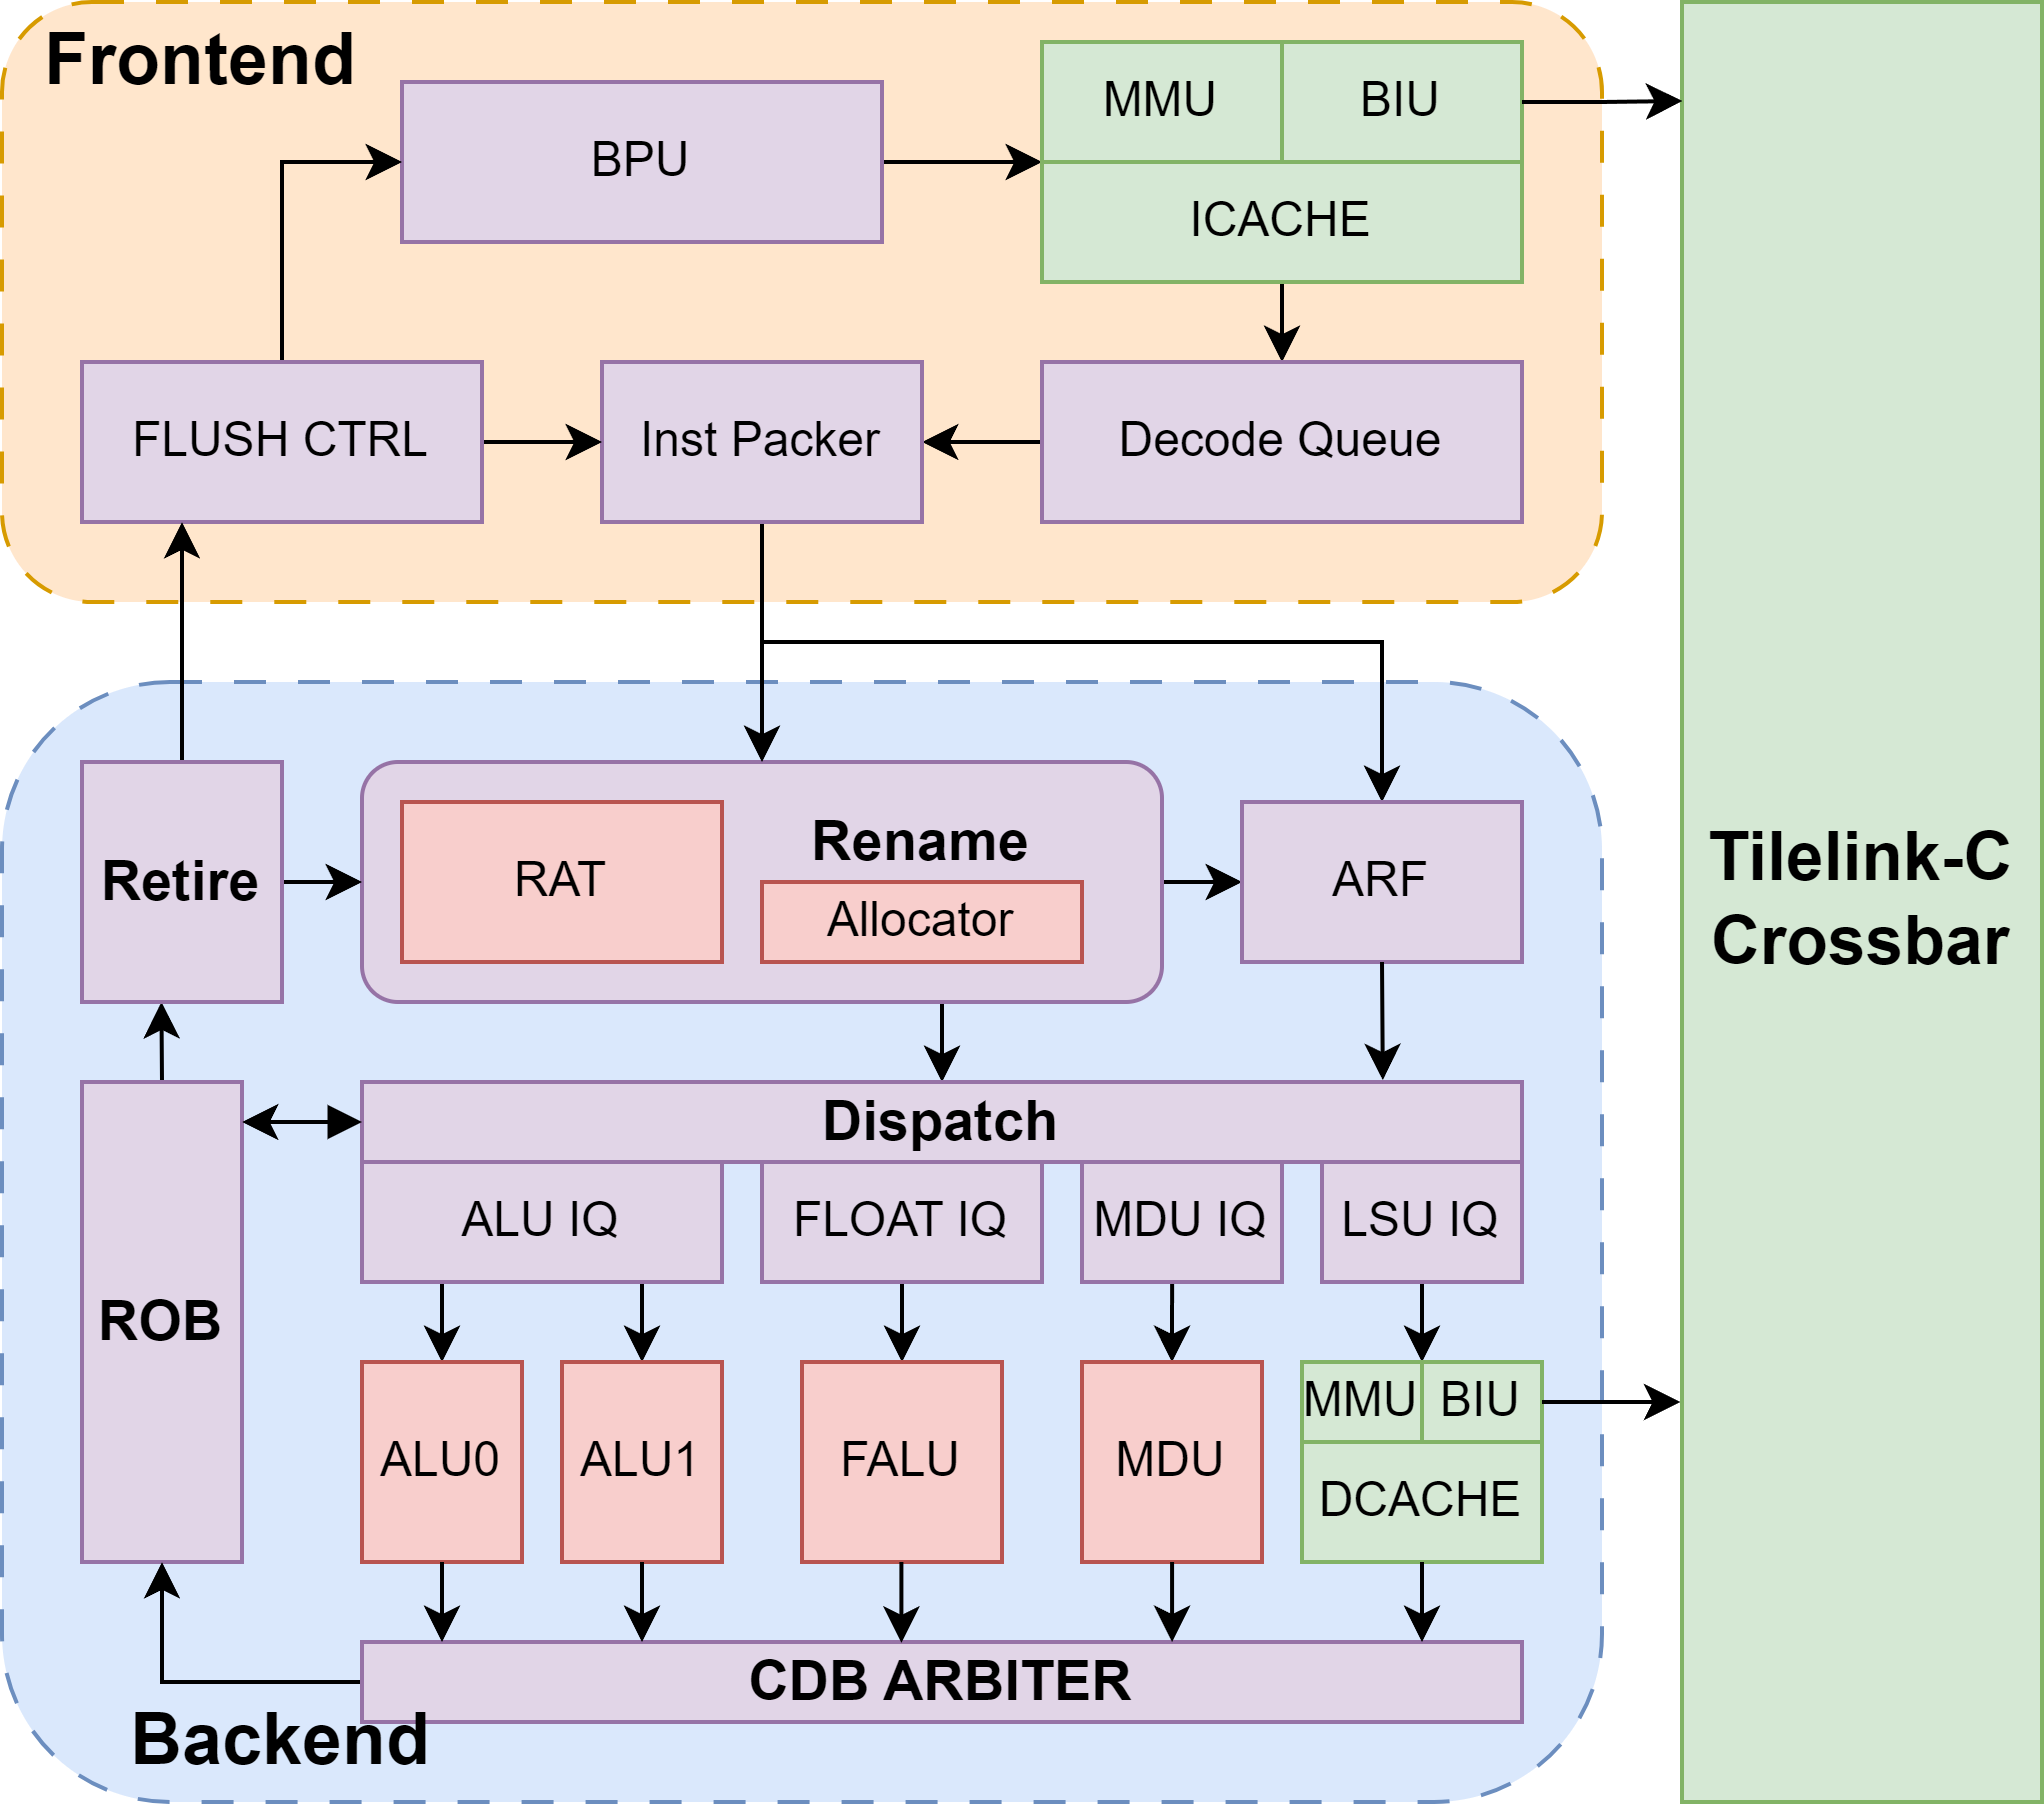
\includegraphics[width=1.0\linewidth]{assets/05/wired-arch.png}
  \caption{Wired 核心整体架构图}
  \label{fig:05-wired-arch}
\end{figure}

\subsection{代码仓库导读}\label{sec:05-complex-cpu-002}

\href{https://github.com/gmlayer0/wired}{Wired232v1} 使用 Systemverilog 实现，全部硬件源码，包括第三方开源 IP ，均存放在 ./rtl 目录之下。

而在 ./src 目录之下存放了一些工具脚本，这里对其代码结构进行简单介绍。

\subsection{工具脚本说明}\label{sec:05-complex-cpu-003}

\begin{itemize}
\item
  ./src/compile\_project.py

  Wired Core 采用的一套 python 脚本，会读取环境变量中的 \texttt{CHIPLAB\_HOME} 并将核心部署到其环境中用于仿真。 其还使用 compile\_settings.json 对使用的模块版本进行管理，每个模块的文件头部会用特殊语法标记其版本， 并在 compile\_settings.json 中实际选择使用的版本。 描述语法形如：

  % 代码语言：BookSystemVerilog
\begin{CodeBlock}[language=BookSystemVerilog]
/*--JSON--{"module_name":"core_lsu_rport","module_ver":"2","module_type":"module"}--JSON--*/
\end{CodeBlock}

  这里描述了一个名为 \texttt{core\_lsu\_rport} 的模块，其版本号为 2，类型为模块（module）。
\item
  ./src/gen\_sram\_wrapper\_*.py

  Wired Core 的设计考虑在不同的平台中使用（仿真器环境、FPGA 环境、流片环境）。在不同环境下，核心需要使用不同的模块作为存储器使用。

  好在 Wired Core 设计中只使用了单口及双口的 sram，而 sram 在不同平台下具有相似接近的行为，仅存在模块名和接口名称的区别。

  因此我们使用这样一个小工具，生成我们需要使用的，兼容不同平台，不同容量 sram 的生成工具生成核心使用的 sram。
\item
  ./src/inst

  Wired Core 支持使用一套 python 脚本生成核心使用的解码器及相关指令静态控制信息。这套工具使用一组 json 描述指令集。

  在 \texttt{./src/inst} 目录中，存放默认使用的 la32r 整数指令集解码信息。其中 \texttt{general.json} 定义一些常量，以及处理器流水线通用的一些控制信号，及流水级顺序。

  对于常量的定义，直接使用一个键值对即可，由常量名映射到其值。这部分会被使用 \texttt{\textasciigrave{}define} 定义成常量使用。

  形如：

  % 代码语言：BookJSON
\begin{CodeBlock}[language=BookJSON]
"_REG_R0_IMM": "2'b11"
\end{CodeBlock}

  等价于 \texttt{\textasciigrave{}define\ \_REG\_R0\_IMM\ 2\textquotesingle{}b11}
\end{itemize}

对于流水线的定义，采用一系列二元组，描述流水线关系的 DAG 图，形如：

% 代码语言：BookJSON
\begin{CodeBlock}[language=BookJSON]
[
        ["alu", "c_alu_common"],
        ["c", "c_alu_common"],
        ["rob", "c"],
        ["p", "alu"],
        ["p", "rob"],
        ["d", "p"],
        ["Entry", "d"]
]
\end{CodeBlock}

关于流水线控制信号定义，也使用一个键值对的格式描述，如：

% 代码语言：BookJSON
\begin{CodeBlock}[language=BookJSON]
"imm_type": {
    "length": 3,
    "stage": "is",
    "default_value": "`_IMM_U5"
}
\end{CodeBlock}

这组定义描述了一个信号名为 \texttt{imm\_type}，且会在 \texttt{is} 级使用（之后流水级不使用）的控制信号。其长度为 3，默认值（不手动指定时）为字符串 \texttt{\textasciigrave{}\_IMM\_U5}

控制信号会按照其不同流水线位置，分布在不同流水级之间，并自动生成流水控制信号在各级别之间传递转换的函数。

在其它 \texttt{.json} 文件中，描述了指令使用的具体解码信息，及部分专用指令控制信号，形如 \texttt{alu.json} 中对于 \texttt{add.w} 指令的定义：

% 代码语言：BookJSON
\begin{CodeBlock}[language=BookJSON]
"add.w": {
    "opcode": "00000000000100000",
    "alu_grand_op":"`_ALU_GTYPE_INT",
    "alu_op":"`_ALU_STYPE_ADD",
    "reg_type_r0": "`_REG_RK",
    "reg_type_r1": "`_REG_RJ",
    "reg_type_w": "`_REG_W_RD",
    "alu_inst": 1,
    "das": "\"$r%02x, $r%02x, $r%02x\",rd, rj, rk"
}
\end{CodeBlock}

其中， opcode 字段定义了指令的解码信息。大部分 LA32R 指令采用可变长的前缀解码的形式，因此只用在 opcode 中描述其前缀码即可。对于解码时不关心的位，可以使用 x 跳过，如下指令。

% 代码语言：BookJSON
\begin{CodeBlock}[language=BookJSON]
"bcnez": {
    "opcode": "010010xxxxxxxxxxxxxxxx01",
    "fbranch_inst": 1,
    "bcnez": 1,
    "cmp_type": "`_CMP_E",
    "target_type": "`_TARGET_REL",
    "jump_inst": 1,
    "das": "\"%07x\",I26<<2",
    "fpd_inst": 1,
    "slot0": 1
}
\end{CodeBlock}

\section{重命名实现}\label{sec:05-complex-cpu-004}

Wired 核心的寄存器重命名采用基于 ROB 的策略。在指令解码得到指令信息之后，来到重命名级别。

重命名级别内部拥有三张表（由寄存器堆实现），三张表分别命名为 Rename 级重命名映射表（以下简称 Rename 级表）、 Commit 级重命名映射表（以下简称 Commit 级表）、TierID 表。 对寄存器的重命名操作，就依赖对这几张表的查找和更新操作。其中，Rename 级表的写口由重命名级输入的写寄存器号控制，用于更新记录在 Rename 阶段为写寄存器分配的重命名寄存器号。 Commit 级表则用于记录提交时的状态更新。

在重命名级别，指令需读取的体系结构寄存器号会被用于访问这数张表，拿到其在 Rename 阶段及 Commit 阶段分别对应的重命名寄存器号及 TierID。 其中 Rename 级重命名映射表中存储的重命名寄存器号即为相应寄存器的最后一次重命名分配结果，而 Commit 级重命名映射表则存储了相应寄存器上最后一条被提交的重命名分配结果。 当两个重命名寄存器号一致时，说明此时后端流水线中对该读寄存器最新的一次写入操作已经退休，即该寄存器对应的最新值已被写入 ARF 中。 否之则相应指令还没有退休，仍位于 ROB 中，或者管线里面。

这样的设计存在一个缺陷：假如某轮重命名过程中，分配给指令的重命名寄存器号与上一次提交时分配的重命名寄存器号恰好一致，则重命名表与提交表中会记录相同的寄存器号。 此时，虽然最新的对该寄存器的修改指令还没有退休生效，ARF 中的值并不是有效的最新值，但后续指令可能会由于表的错误状态，错误判断数据位置。

TierID 表就是设计用于回避这种情况。每次在重命名更新 Rename 级重命名映射表时，会将 TierID 表中存储的旧 TierID 读出，并取反作为重命名后最高位的 TierID。 在提交级，将该 TierID 再写入 TierID 表。 由于 TierID 在重命名级时，需要访问四个读寄存器号对应值，以判断 ARF 中的数据是否有效。 同时，还需要访问两个写寄存器号对应值，以保证重命名后寄存器号一定不同，因此单独实现提交级的 TierID 表，而不是与 Commit 级重命名映射表共用。

\begin{figure}[htbp]
  \centering
  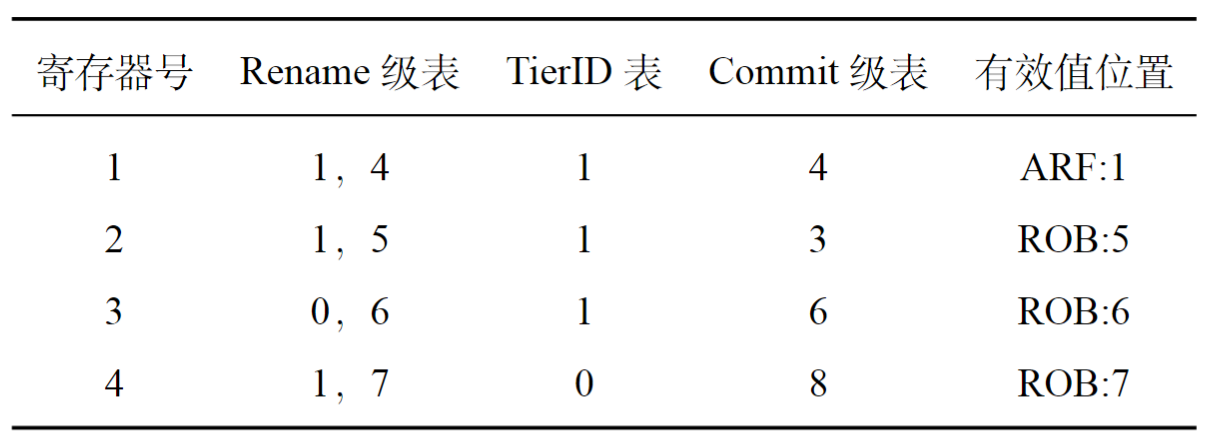
\includegraphics[width=1.0\linewidth]{assets/05/rename-showcase.png}
  \caption{某时刻部分重命名表项状态}
  \label{fig:05-rename-showcase}
\end{figure}

如图\ref{fig:05-rename-showcase}中描述了某一时刻重命名的三张表中存储的四个寄存器重命名状态。 其中可以发现，对于一号寄存器，其 Rename 级表中记录的 TierID 与 TierID 表中记录的一致，且重命名寄存器号也与 Commit 级表中的一致，说明该指令的修改已被提交到 ARF，ARF 中一号寄存器的值就是最新的有效值。 对于二号寄存器，其 Rename 级表记录的 TierID 与 TierID 表中记录的一致，但重命名寄存器号与 Commit 级表记录不同，说明最后一条写入该寄存器的指令尚未提交，且相关指令被重命名为 ROB 中的五号寄存器。 对于三号寄存器，四号寄存器也进行相同的分析，可以发现其最新值均位于 ROB。以上就是重命名状态表的一次完整查找流程。

重命名模块内部还会维护 ROB 的指针，和 ROB 空闲表项计数。 当且仅当 ROB 空闲表项大于等于发射宽度时，重命名分配级才能继续工作。对于 ROB 的退休，提交级会把退休信号接入重命名模块，以供重命名模块维护更新空闲表项计数等。

\section{ROB 实现}\label{sec:05-complex-cpu-005}

ROB 是流水线后端的关键模块，负责记录尚未退休（提交）的指令控制信息及数据信息，也是正确理解乱序执行体系结构设计思路的关键。

ROB 设计上使用 Bank 策略的多个寄存器堆实现。将多读口一写口（xr1w） 的寄存器堆以 Bank 方式组成多读口多写口（xryw） 的多写寄存器堆。 整个 ROB 使用了四个双写口（双 Bank）的寄存器堆，但其具有不同的读口数量，以及不同的读写控制信号接线。

\subsection{ROB Static 表}\label{sec:05-complex-cpu-006}

ROB Static 表采用一个两读两写的寄存器堆实现，被用于记录指令通过解码得到的静态控制信息。此寄存器堆的两个写口连接到分发级，分别用于写入两条被分发的指令的静态控制信息。 两个读口则接入提交流水线，用于在指令提交时读出指令的静态控制信息。 目前的这种设计，允许每周期向 ROB 写入两条指令，完成两条指令，构成流水线的最窄宽度。在写入时，由于相邻两条指令其重命名后的寄存器号一定具有不同的奇偶性，在写入 ROB 时一定不会冲突。

\subsection{ROB Valid 表}\label{sec:05-complex-cpu-007}

ROB Valid 表用于记录 ROB 表项中的数据是否有效，对于分发级刚写入 ROB 的表项，其 Valid 需要被清空，而 CDB 写回 ROB 的数据，则需要被标记为有效。 由于处理器 CDB 每周期支持完成两条指令，分发级也支持两条指令的分发，因此这里的实现实际上需要做一个四写口的寄存器堆，分别允许在分发级置0及在提交级置1。

对于其读端口，分别需要在分发时读取 ROB 中数据是否有效，提供四个读口、在提交时检查 ROB 中数据是否有效，提供两个读口，总计六个读口。 实际在 Wired 的实现中，使用两个八读口双写口的寄存器堆采用 XOR 的策略拼接完成此多写口的寄存器堆。对于读取，实际六个读口的读输出配置为两个寄存器堆八读口中的六个读口输出值的异或。 对于写入，则分别将清空和置位的控制信号接入两个不同寄存器堆的写口及对位寄存器堆的剩余两个读口。对于清空寄存器堆写入的数据信号，接自对位寄存器堆的读口，对于设置寄存器堆写入的数据信号，则接自对位寄存器堆的读口取反。 这样实现，保证清空写入后，对应某ROB项的两个寄存器堆读出值一定一致，异或值为0。置位写入后，对应某ROB项的两个寄存器堆读出值一定不同，异或值为1。借用两个双写口寄存器堆实现四写口寄存器堆，优化资源占用情况。

\subsection{ROB Data 表}\label{sec:05-complex-cpu-008}

ROB Data 表用于记录指令执行结果。其拥有两个写口供 CDB 使用，写入指令执行后的数据情况。拥有六个读口，四个用于分发时获得 ROB 数据，两个用于提交时获得 ROB 数据。 整个表采用与 Static 相同的设计思路，不同之处在于其两个写口直接连接到 CDB，而 CDB 连接到多个功能单元。 这里就为 CDB 引入了一个限制，即 CDB 每周期仅能接受一奇一偶两个写入 ROB 的请求。对于超过两个的请求，或者超过一个的奇或偶请求，都不能在一个周期内完成响应，需要进行仲裁与等待。

\subsection{ROB Dynamic 表}\label{sec:05-complex-cpu-009}

ROB Dynamic 表用于记录指令的动态控制流信息，包括跳转情况和异常情况。其拥有两个写口供 CDB 写入使用，写入执行后才能够确定的指令情况。拥有两个读口，用于提交时获取指令的控制流信息，也因此与 Data 表存在差异，读口少了四个。 在写口实现方面， Dynamic 表与 Data 表采用了相同的策略，需要进行仲裁与等待，可以与 Data 表完全同步。

\subsection{CDB 实现}\label{sec:05-complex-cpu-010}

前文提到，Wired 中采用的 CDB 每周期仅能提交一奇一偶两条对 ROB 的写回请求。因此 CDB 需要在众多功能管线之间进行仲裁，选择两条请求提交。 Wired 先对所有管线的请求进行了``扩充''，即按照其目标 ROB 地址的奇偶性，将请求一分为二（自然，其中仅会有一个请求是有效的）。 这样一来，即可对所有为奇或为偶的请求，各自进行一次仲裁，得到两个 CDB 上被接受的请求。 根据这个特性，CDB 也被分为固定的一奇一偶，所有偶请求，仅会在第一个 CDB 上出现，而所有为奇的请求，仅会在第二个 CDB 上出现。这种设计，也一定程度上简化了 CDB 监听时的逻辑复杂度和负载，提高了设计频率。

\subsection{ROB 退休}\label{sec:05-complex-cpu-011}

指令退休阶段存在三级流水，分别用于读取 ROB、检查指令情况、执行写入等影响体系结构状态的操作、完成 ARF 更新及跳转更新三个阶段。 读取 ROB 部分的逻辑比较简单，根据 ROB 部分传出的有效性，和后级流水的就绪情况，更新 ROB 读指针，并利用 ROB 读指针从 ROB 读取出数据，送入后端流水处理即可。 特别的，对于 CSR 读取，也在指令退休阶段进行处理。在第一阶段流水，读取 ROB 的同时，会将 ROB 中存储的 CSRID 用于读取 CSR，并在下一周期返回读取结果，供提交更新使用。

在 Wired 的设计中，频繁使用了刷新流水线的形式解决复杂的控制相关问题。对于 CSR / TLB 或者分支误预测，写缓存缺少，不可缓存读取，不可缓存写入，以及推测唤醒的错误恢复，均使用刷新流水线解决。 在流水线刷新后，后端所有未提交的指令被清出流水线，重命名映射表被复位到初始状态，即所有寄存器的最新值均在体系结构寄存器堆中。体系结构寄存器堆不用做特别处理，其已经是体系结构中最新的状态了。

检查阶段有一个重量级的组合逻辑，用于检查指令状态，并完成一些特殊的指令提交检查逻辑。 指令首先会被检查是否触发了异常或者出现了错误的分支预测。对于这一类指令，会立即更新 CSR，并向前端发出控制流重定向请求以更新状态。 完成控制流检查后，指令是否需要被执行的情况已经被确定。之后对于所有需要提交的访存指令，会进一步开展访存情况检查。 对于不可缓存类型的指令，在这里会给访存模块发出处理请求，并等待处理完成。对于可缓存的指令，若是读指令，检查是否出现了错误的推测唤醒。 若发生错误推测唤醒，则需要清空流水线。若是写指令，检查其访存模块中 store buffer 的状态，检查是否命中。若不命中，进行重填，否之弹出 store buffer 表项完成更新。 对于原子写入指令，若不命中，则判定指令执行失败，设定执行失败，并刷新流水线。

对于 CSR/TLB 的更新操作，也在这里完成。对 CSR / TLB 完成刷新后，对应会重启流水线，以保证其影响能够被后续指令观察到。不可缓存的操作 也在这里开始实际执行。 由于部分指令直到提交阶段才能确定其执行结果，这部分在提交阶段指令执行结果错误的指令，可能会错误的导致后续指令观察到错误的值。 但体系结构寄存器堆中的值，始终都是有效的。因此，对这些指令，也会强制刷新流水线，并将正确的值写入体系结构寄存器堆，以消除错误的值造成的影响。

\section{指令发射及唤醒实现}\label{sec:05-complex-cpu-012}

指令完成重命名及 ARF 读取后，会来到分派级被分派到各个发射队列。 流水线后端的所有执行单元，则由各个发射队列（Issue Queue 简称 IQ）直接控制。 发射队列采用分布式设计，整体分为整数指令/访存指令/乘除指令/浮点运算/浮点分支五类发射队列。 其中整数、乘除指令、浮点运算的发射队列支持乱序执行，而访存指令为了保证处理器系统的 TSO 内存一致性并降低设计复杂度则是顺序发射。浮点分支指令为了保证分支正确性降低复杂度，也使用顺序执行策略。 指令在各自的发射队列中会持续监听所有操作数状态，等到所有需要的操作数就绪后指令就可以发射。

指令发射逻辑经过专门优化，保证所有指令是否能发射的控制信号直接来自一个寄存器，以降低后续发射选择及唤醒逻辑的逻辑复杂度。 由于指令完成，到指令执行结果出现在 CDB，并反馈到发射队列存在数个周期的延迟，为了支持指令背靠背执行，降低执行延迟，部分发射队列还做了对唤醒逻辑的实现，允许指令在数据没有就绪（但能保证在数据被使用时一定就绪）时提前发射。 整个处理器采用相同的唤醒接口，每个唤醒源产生唤醒有效、唤醒重命名寄存器号、唤醒数据这三个信号。在唤醒有效拉高后的第二个时钟周期，一定会得到有效的唤醒数据。被唤醒方只需要按照这个时序条件接受唤醒源，并及时进行数据转发即可完成。

所有执行管线均采用相同定义的接口与发射队列及通用数据总线连接，以降低设计复杂度，提高设计复用率。 执行管线输入输出各自使用一套 Valid-Ready 机制进行握手，当输入握手成功时，指令执行需要的操作数及控制信号已经就绪。当输出握手成功时，指令执行的结果已经就绪，送入 CDB 仲裁等待写回 ROB。 对于执行管线的有序性，也并不做要求，指令可以以任意的顺序被完成。如对浮点 ALU 单元，指令被按序请求执行，但不保证按序完成。指令控制信号中会包含指令重命名后的寄存器号（ROB ID），用于产生写回 ROB 时的写地址。

由于这样一套接口定义，核心在执行管线方面成功实现了较好的解耦合。各个模块之间的耦合度较松，也可以通过插入 先入先出队列 或者流水线寄存器等方式，实现弹性流水线以优化吞吐量和核心频率。 执行管线方面，如管线长度等细节，也实现了对发射队列及后端提交流水线的完全隐藏，降低处理器调试复杂度。

具体执行管线方面，对于简单整数 ALU 的实现比较简单，使用多个 Mux 输出不同结果即可。 对于乘法器，由于现有综合器已经有较好的综合优化性能，无论在 FPGA 或者流片上面，都能综合出较为高效的电路，Wired使用乘法符号生成乘法器，交由编译器自行完成优化。 Wired 也在乘法器输入输出上均额外添加一级流水，以优化频率性能。对于除法器，Wired采用了非恢复余数除法器，可以在32个周期内完成除法的计算。 浮点方面，处理器核将浮点指令按照是否需要按需完成（涉及条件控制位 cc），分为浮点分支指令及浮点计算指令。 对于浮点分支指令，指令全部按序发射，按序执行，耗费一个时钟周期，完成浮点比较，浮点分支，浮点条件选择等浮点控制标志位（fcc）相关的指令功能。 浮点计算指令复用开源项目cvfpu，提供了大部分 LA32R 所需要的浮点计算指令支持。 对于少部分 LA32R 支持，而 cvfpu 不支持的指令，如 frsqrt.s、fmaxa.s、fmina.s 经过对编译器的检查，发现其不会自动推断出这些指令。因此也没有进一步提供支持。 浮点指令还有一类比较特殊的三读寄存器指令，即浮点的乘加指令。对于这类指令，需要考虑在一周期内向其提供三个寄存器的读支持。 因此，Wired扩充了访存期间，第一条流水线访问操作数的通路，到三条，允许每周期捕获三个操作数。

\section{访存子系统实现}\label{sec:05-complex-cpu-013}

访存子系统的具体设计，将在本节进行详细的介绍。

\subsection{整体概览}\label{sec:05-complex-cpu-014}

访存子系统的设计实现是正确处理内存一致性问题及缓存一致性问题的关键。 Wired实现了使用 Tilelink-C 作为总线协议的访存子系统。 LA32R 中的浮点及整数单元共用这个访存子系统。 访存子模块需要以较高吞吐量、较低延迟响应来自核心的访存请求，并保证多核心之间的缓存的一致性行为及内存一致性约束。 此设计中的访存子模块，整体可抽象为如图\ref{fig:05-tso-maintain}中的结构。 其按照 TSO 的内存一致性约束进行设计，接受并执行来自发射队列顺序发射的所有访存指令。 对于写指令，访存子系统将其存入前递写缓冲（Forwarding Store Buffer）而不立即写入存储器。 对于读指令，保证其执行顺序与程序顺序一致。这样一来，对于本核心的所有写入和读取操作，在本核心看来依然满足程序语义顺序。 其它核心视角看到，会发现本核心写入与读取操作之间可能没有保持程序语义中的约束，但不同的读请求之间及不同写请求之间依然保持了程序语义的顺序。

\begin{figure}[htbp]
  \centering
  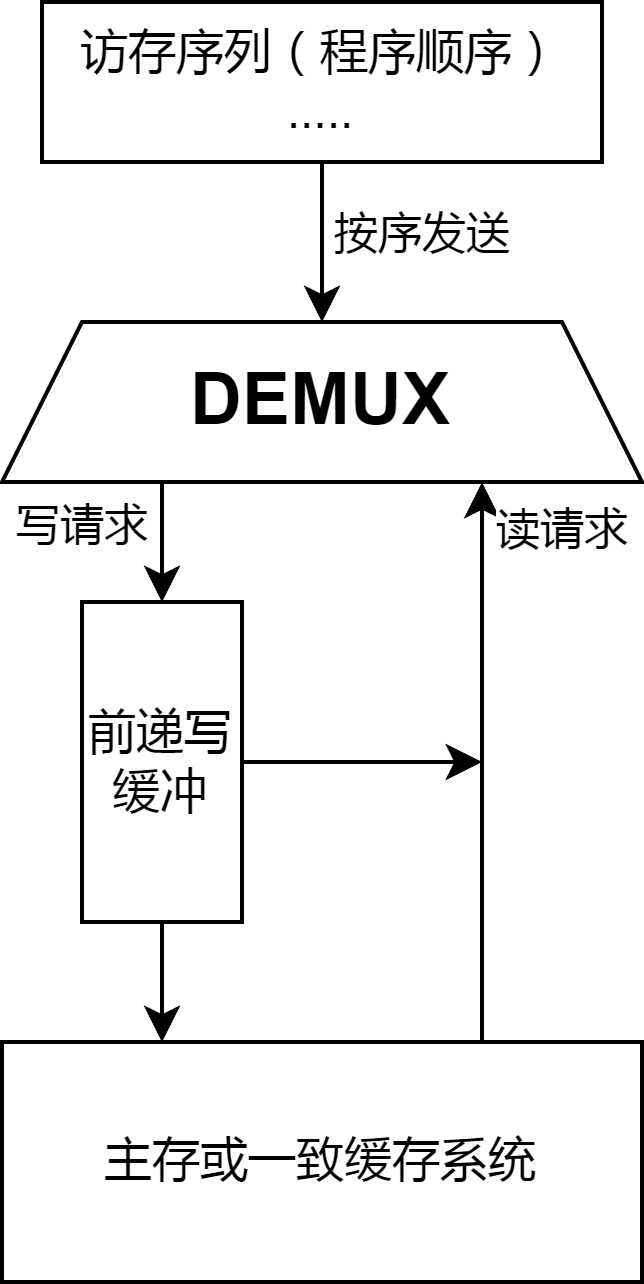
\includegraphics[width=0.25\linewidth]{assets/05/tso-maintain.png}
  \caption{访存子系统抽象结构}
  \label{fig:05-tso-maintain}
\end{figure}

\begin{figure}[htbp]
  \centering
  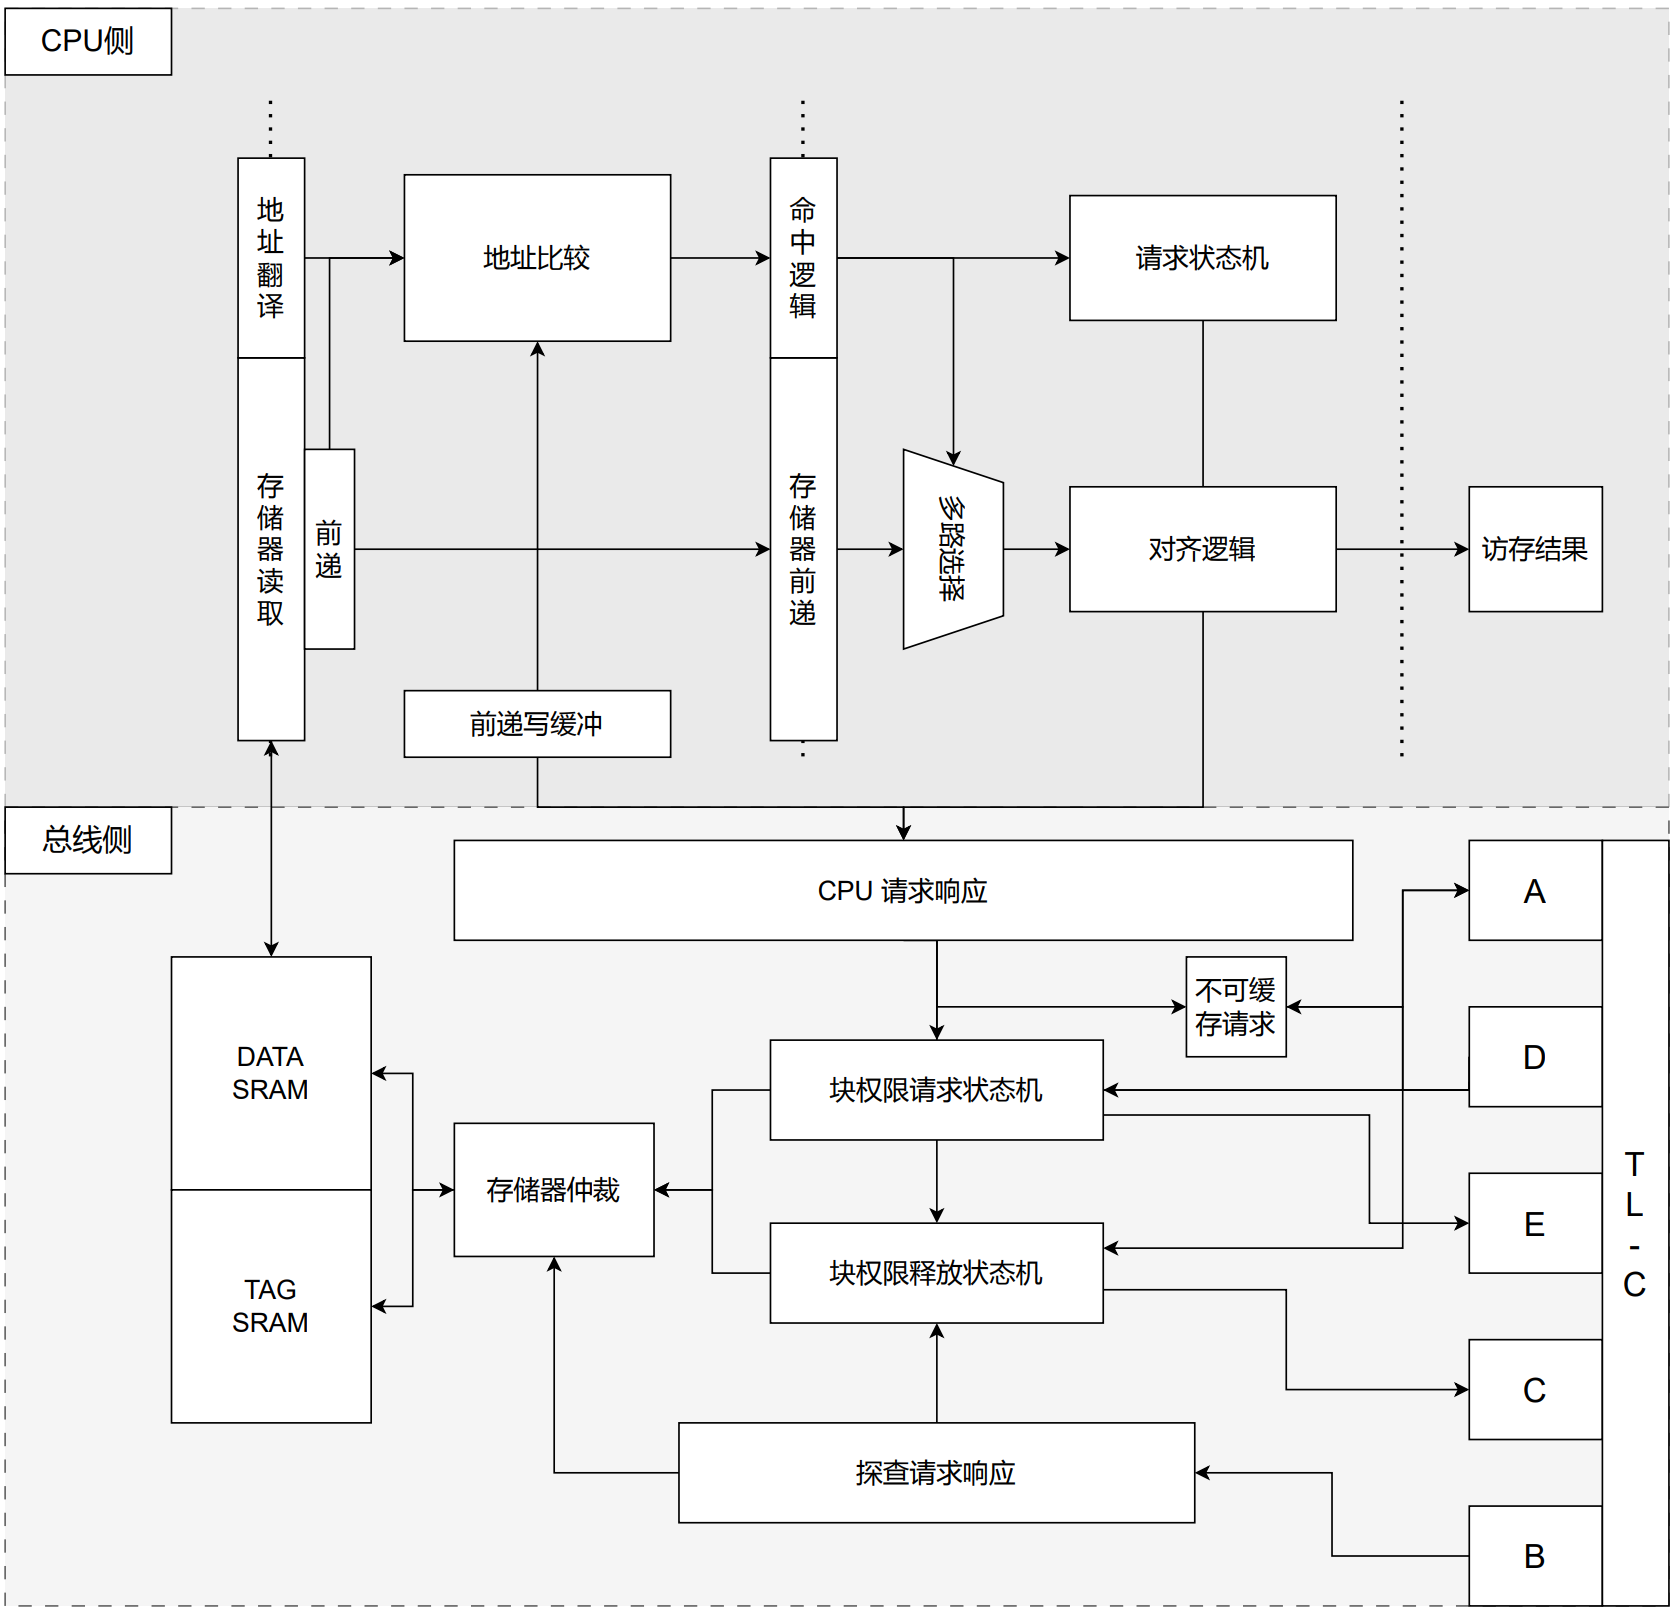
\includegraphics[width=1.0\linewidth]{assets/05/cache-subsystem.png}
  \caption{整体访存架构}
  \label{fig:05-cache-subsystem}
\end{figure}

这种实现可以优化处理器性能（减少推测写入错误后带来的额外恢复开销），并且避免进行激进的访存乱序检查，简化实现复杂度。 对于软件方面的实现，TSO 内存一致性接近顺序一致性模型，可以减少软件方面的系统设计复杂度。 为了实现对称多核系统，访存子模块中的缓存需要支持缓存一致性协议，以保证多个核心中缓存的数据一致性。 具体来说，Wired使用 Tilelink-C 实现了一套 MSI 的缓存一致性协议。 每个缓存行存在三种可能状态，分别是独占修改、共享无修改、无效。通过保证系统中时刻只存在一个写者或多个读者，保证了系统中多个缓存系统的一致性。

具体到缓存的设计，整体设计被分离为 CPU 侧以及总线侧两部分以简化复杂度。 整体模块如图\ref{fig:05-cache-subsystem} 所示。 总线侧负责产生并处理所有 Tilelink-C 的消息，并对数据存储器及 Tag 存储器进行探查与更新。 CPU 侧则拥有数据存储器及 Tag 存储器的读权限，以及对数据存储器的写权限。 对于前递写缓冲中的指令以及 LSU 流水线中的所有其它指令，CPU 侧流水线保持对 Tag 存储器写信号的探查，以实时更新命中或者权限状态。

CPU 侧在未命中或者执行缓存指令时，会向总线侧发出请求以无效化/申请对应的缓存行。 总线侧接受来自 CPU 侧及 Tilelink-C 的请求，完成相应请求的所有总线动作或存储器动作后反馈完成结果给 CPU 侧或 Tilelink-C。 缓存一致性协议及其他总线协议等细节，在总线侧使用多组状态机实现，完全对 CPU 侧保持透明。若希望实现基于 AXI 总线的缓存，亦或是 ACE 总线，均只需要更新总线侧的模块即可。

对于所有访存指令中的读请求，访存子模块会立即检查缓存是否命中并阻塞式的等待重填请求完成以保证拿到所需要的权限。 特别的，对于链式加载（Load-Linked word）指令，缓存会检查并申请写权限以辅助条件写回（Store-Conditional）指令实现。 条件写回指令执行时，会再次确定持有写权限，保证可以不进行重填的完成相关操作。

对于非原子属性的写请求，在缓存中会检查缓存行状态，并将状态保存到前递写缓冲中，同时实时探查总线上的修改并维持更新。 等待写指令提交的时候，会确认写指令对于缓存的命中情况。若缓存命中且持有写权限则完成更新。 否之则会触发缓存的重填和权限申请，等待拿到缓存行的写权限再完成写请求到存储器的提交。 这种实现保证了存储器中的所有值一定不是在推测状态下被写入的。从其它核心角度观察，可能会发现本核心的部分读取请求被提前到写请求之前，这依然满足 TSO 内存一致性的约束。

\subsection{访存 CPU 侧流水线}\label{sec:05-complex-cpu-015}

访存子系统在 CPU 侧有一个三阶段的流水线结构。流水线第一阶段用于地址生成及读存储器，第二阶段用于地址比较及前递写缓存的写入，第三阶段用于缺失处理及数据生成。

第一阶段的实现较为简单，将虚拟地址的低 12 位（4K空间）直接送入存储器，并行读取缓存的数据存储器及 Tag 存储器获取数据及 Tag。 由于 LA32R 设计中，地址翻译的最小粒度为 4K，即任何地址翻译模式下，虚拟地址及相应物理地址的低 12 位均是一致的。虚拟地址的高 20 位将被送入地址翻译模块，在下一周期获得物理地址及相关访问属性。 第二阶段被用于做地址比较检查，使用第一阶段请求的缓存请求物理地址及缓存行中存储的 Tag 信息进行命中检查。对于写请求，会将命中检查后的结果连带请求写入前递写缓存等待提交，并供后续读指令检查。 第三阶段实质上是一个缓存状态机，处理所有缺失情况并负责读数据的生成，整体状态图如图\ref{fig:05-cachepipefsm} 所示。

\begin{figure}[htbp]
  \centering
  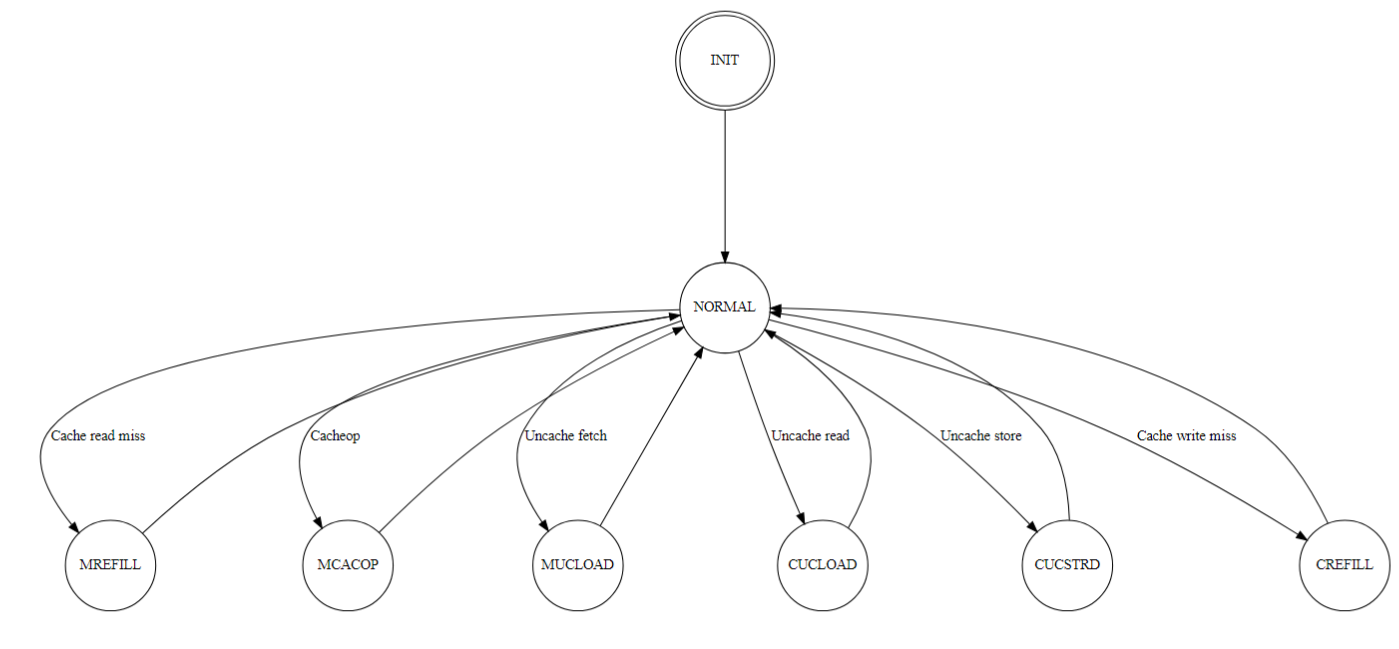
\includegraphics[width=1.0\linewidth]{assets/05/cachepipefsm.png}
  \caption{流水线状态机}
  \label{fig:05-cachepipefsm}
\end{figure}

对于所有写请求，其在流水线的第二阶段被与自己的命中情况一同写入前递写缓存，并时刻监听存储器写总线，维护命中情况的状态。 为了完成写操作的提交，访存子系统向 CPU 提交级保留接口，展示前递写缓存中最旧写指令的状态。提交级的逻辑会进一步交互，如申请对应缓存行写权限，或确认提交，弹出前递写缓存。 根据程序语义，至少在单核心上，所有在某写指令之后的读指令，都应该可以观察到这条写指令的写入效果。 在Wired中，使用前递写缓存维护这一个单核心上的约束。读指令会同时检查缓存行命中情况以及 前递写缓存的命中情况。对于前递写缓存的命中，处理器立即转发相应的转发数据。

对于读取前递的实现，存在一个多命中的问题，即若前递写缓存中存在多条指令写入同一个地址，则后续读指令转发相同地址时应该优先转发最后写入的指令。 这里面存在一个优先级的实现。但优先级的实现往往会产生较大的组合逻辑电路，不利于处理器的频率。Wired为了解决这一点，对前递写缓存做了特殊的优化。所有前递写缓存中的表项都会监听后进入前递写缓存的写指令。 若发生两者写地址重复的情况，则旧表项中用于转发的写位使能信号会更新，保证对于字中的每一个位，在整个前递写缓存中仅存在单个匹配的表项。

缓存中另一个设计的关键问题就是无论在什么情况下（暂停与否），缓存第一级的流水线都需要监听对于缓存存储器的写入，以保证其读到的数据一定是最新的值。 为了实现这个设计，在第一级流水中加入了关于转发的检查，并设计了一个 MUX，用于时刻维护其值最新。此设计同上一章节中介绍的缓存一致。

\subsection{访存总线侧实现}\label{sec:05-complex-cpu-016}

访存子系统的总线侧负责检查 CPU 侧以及 Tilelink 侧的请求，并实现相应的处理。 由于 Tilelink 存在对于通道优先级的要求，在通过 A 通道处理重填任务的同时，可能总线侧也会通过 B 通道发来 Probe 事务。 按照 Tilelink 的规范， B通道上的 Probe 事务需要在 A 通道上的事务没有被响应的情况下也能够被响应。

对于访存子系统的总线侧，整体上有两种实现思路。一种是构建一个非常巨大的状态机，考虑所有可能的 CPU 请求与总线请求组合，以保证满足 Tilelink 约定。 一种是构建多个小的简单事务状态机，分别负责多个不同的子任务，最终联合在一起形成一个巨大的状态机。 考虑到尽可能降低实现上复杂度的需求，Wired决定采用第二种设计思路，即构建多个小的子任务状态机，联合在一起以满足总线侧缓存的功能需求。 具体来说，子任务被拆解到多个子状态机中：

\subsubsection{访存 CPU 响应状态机}\label{sec:05-complex-cpu-017}

CPU 响应状态机处理来自 CPU 侧的重填/无效化/强序非缓存读写请求，并驱动其它子状态机来完成请求。 如对于缓存行的重填请求，CPU 请求响应状态机会先向无效化状态机发出对特定缓存的无效化请求。 无效化状态机中，会检查对应缓存行中的每一路缓存状态，最终选定一行用于重填的路，保证其可被用于重填（不含有有效行，或者含有对应请求的行），返回对应选择给 CPU 响应状态机。 CPU 响应状态机会进一步向权限请求状态机发出请求，提升缓存行权限，并等待重填结果及数据返回，CPU 重填响应状态机将对应状态返回给 CPU 总线，完成重填处理。 对于 Uncached 请求，也是类似的过程。 具体状态转换如图\ref{fig:05-cpureqfsm}所示。

\begin{figure}[htbp]
  \centering
  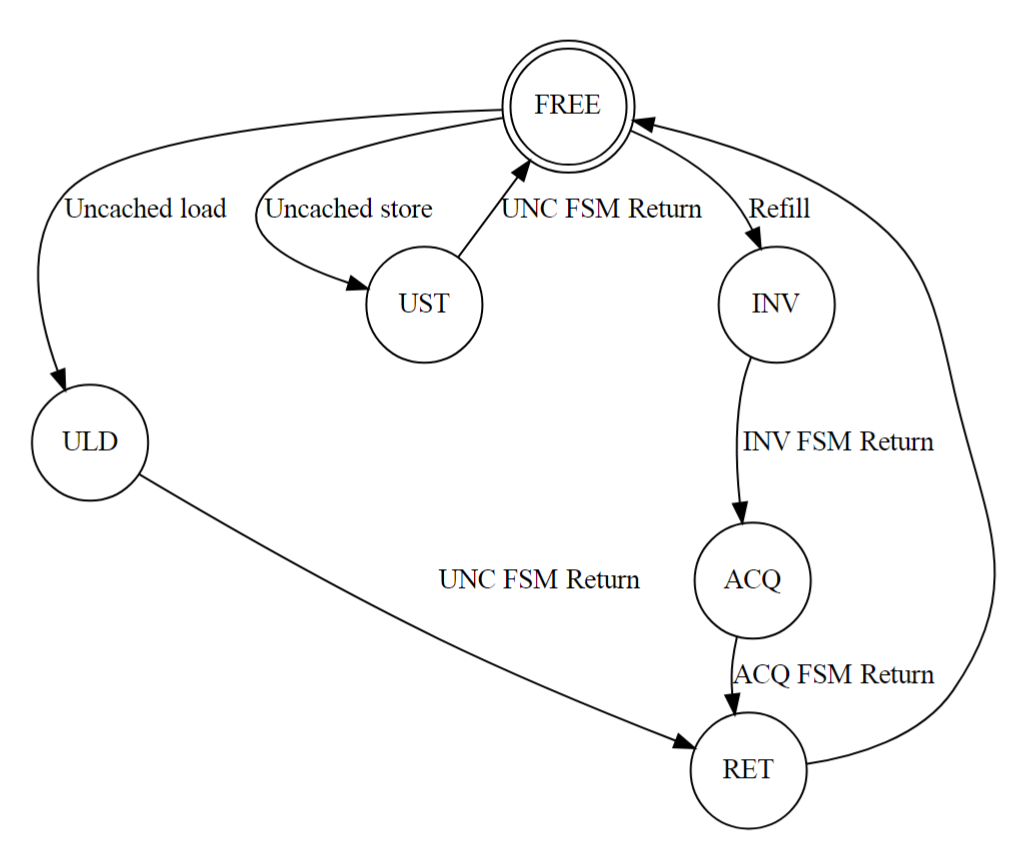
\includegraphics[width=0.5\linewidth]{assets/05/cpureqfsm.png}
  \caption{CPU 响应状态机}
  \label{fig:05-cpureqfsm}
\end{figure}

\subsubsection{Probe 响应状态机}\label{sec:05-complex-cpu-018}

Probe 响应状态机响应来自总线 B 通道的 Probe 请求，并将相应请求交由 INV 状态机完成处理。 需要注意的时候，总线上的 Probe 请求发出的时机是任意的，Probe 响应状态机收到 Probe 的请求同时，INV 状态机可能正在响应来自 CPU 侧的重填请求，这时候 Probe 状态机需要等待 INV 状态机接受自己的请求再继续工作。 对于原子指令对 ll-sc，同一个锁资源可能会在多个核心之间被激烈的竞争，形成资源活锁，最终没有核心能完成原子请求。 为此，该状态机会在 Probe 阶段对上次重填请求的地址加以记录维护。 在上次重填完成的 64 个周期之内，不允许该缓存行被无效化，以解决资源过于激烈的竞争情况。 具体状态转换如图\ref{fig:05-prbfsm}所示。

\begin{figure}[htbp]
  \centering
  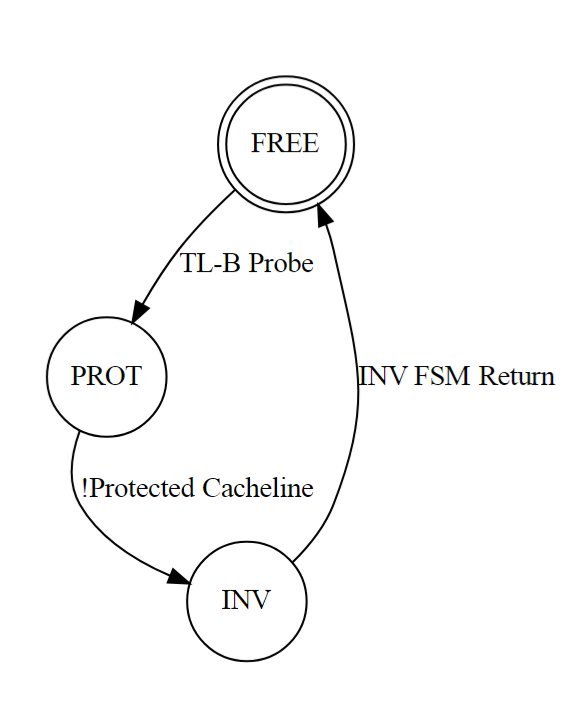
\includegraphics[width=0.35\linewidth]{assets/05/prbfsm.png}
  \caption{仲裁 Probe 响应状态机}
  \label{fig:05-prbfsm}
\end{figure}

\subsubsection{无效化状态机}\label{sec:05-complex-cpu-019}

无效化状态机接受来自 CPU 响应状态机及 Probe 响应状态机的请求，按照需求检查缓存行状态，降低或无效化缓存行权限，并向总线或 CPU 响应状态机反馈无效化情况。 这个状态机较为复杂，需要处理包括重填无效化 / Cacheop 无效化 / Probe无效化 在内多种情况，还需要考虑对脏数据的写回问题。 具体状态转换如图\ref{fig:05-invfsm}所示。

\begin{figure}[htbp]
  \centering
  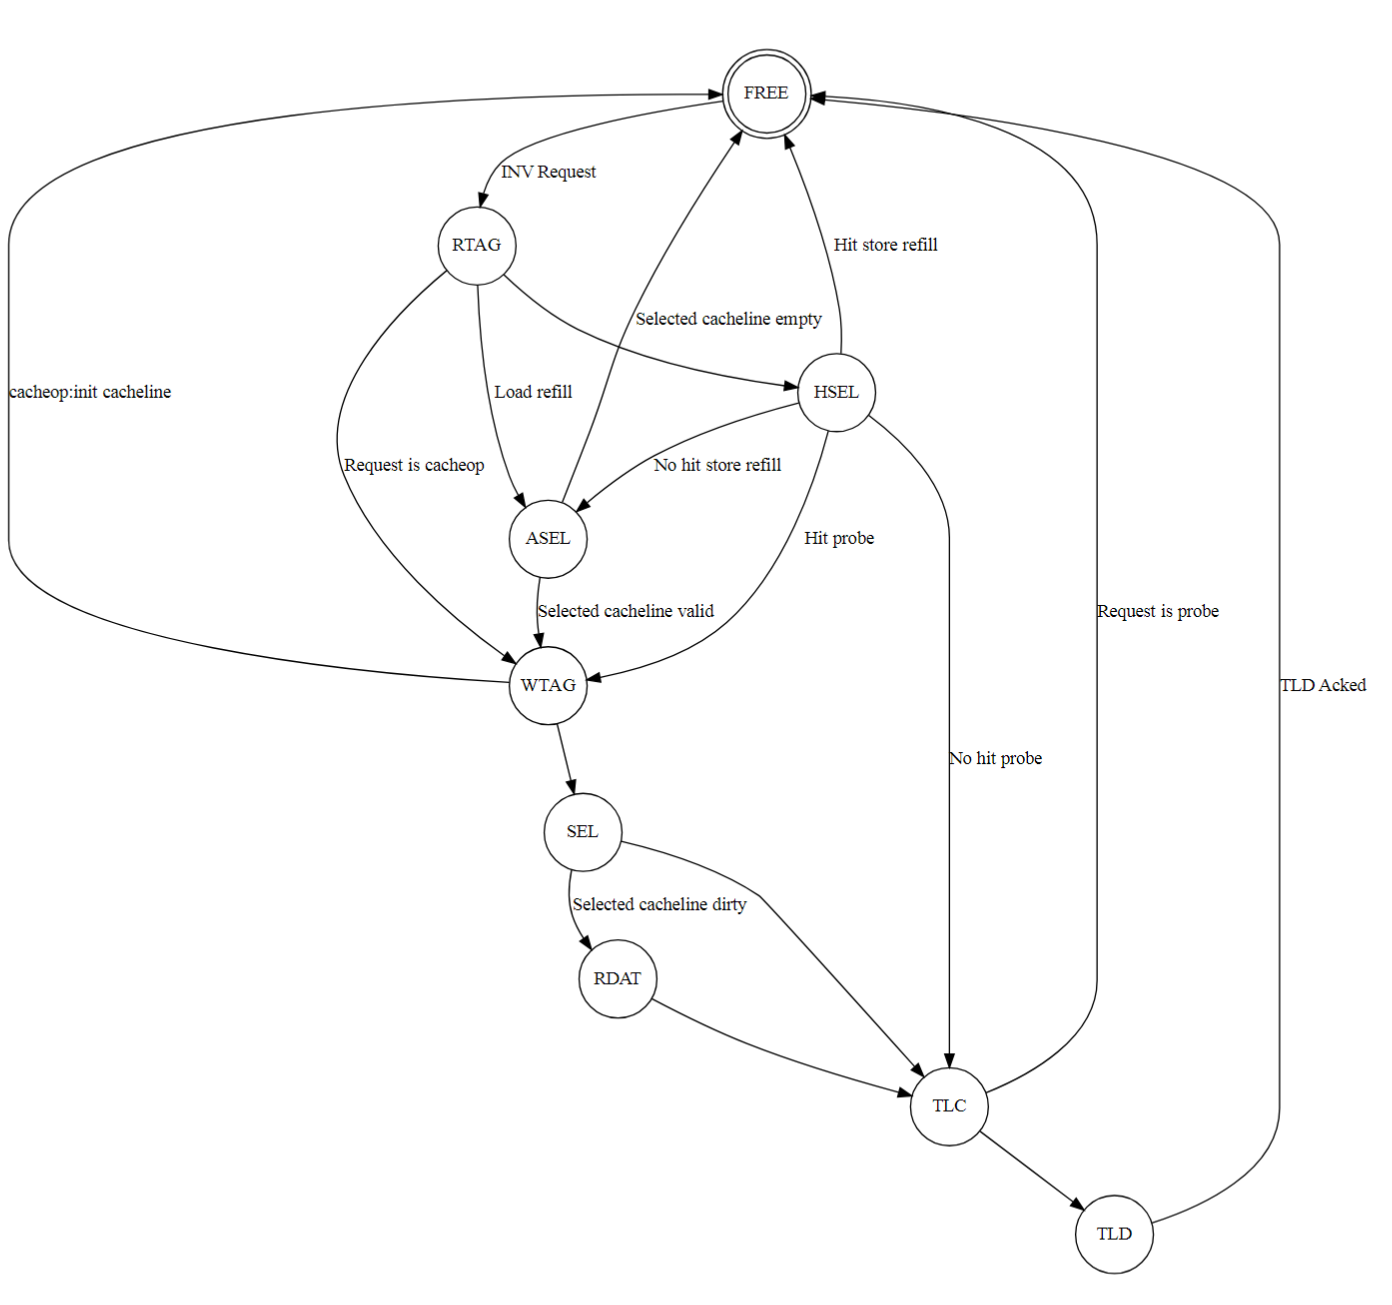
\includegraphics[width=1.0\linewidth]{assets/05/invfsm.png}
  \caption{无效化状态机}
  \label{fig:05-invfsm}
\end{figure}

整体上来说，对于所有请求，会先读取其缓存行的 TAG，之后对 TAG 做检查，判定是否需要无效化，以及需要无效化哪些行。 对于无效化的操作，还需要通过 Tilelink 总线告知父亲一致性节点以辅助进行 Snoop Filter 的操作。 对于缓存存储器的访问，在缓存总线侧的多个状态机之间，存在仲裁关系。 因此对于无效化状态机，其对缓存存储器的读写请求，不一定保证能够满足，因此所有与存储器相关的状态（RTAG、WTAG、RDAT）均会等待存储器就绪，可以响应请求之后才继续进行到下一状态。

\subsubsection{权限请求状态机}\label{sec:05-complex-cpu-020}

权限请求状态机接受来自 CPU 响应状态机的请求，向 Tilelink 总线请求对应缓存行的权限及数据，并写入缓存存储器。 在调用权限请求状态机时，需要重填的缓存行已经经过 INV 状态机处理，一定是空的状态，因此权限请求时不用处理回填的情况，只需要从总线获取数据和权限，更新缓存的存储器即可。 具体状态转换如图\ref{fig:05-acqfsm}所示。

权限请求在 Tilelink 的规定中，通过 TL-A -\textgreater{} TL-D -\textgreater{} TL-E 的三次握手完成。因此权限请求状态机就是负责在这三个总线通道上进行数据的交互，完成缓存行数据获取及权限提升的操作。 与无效化状态机一样，权限请求状态机对于缓存存储器的读写请求也需要仲裁，不一定能被满足。这里存在一个约束就是对于 TAG 的写入一定不早于对 DATA 的写入，否之可能会导致流水线中读到缓存存储器中错误无效的 DATA 数据。 这里实际的实现是先发出对 DATA 的写入请求，直到 DATA 允许写入之后才允许向 TAG 发出写入请求。当 TAG DATA 均完成写入后才认为这次权限请求完成。

\begin{figure}[htbp]
  \centering
  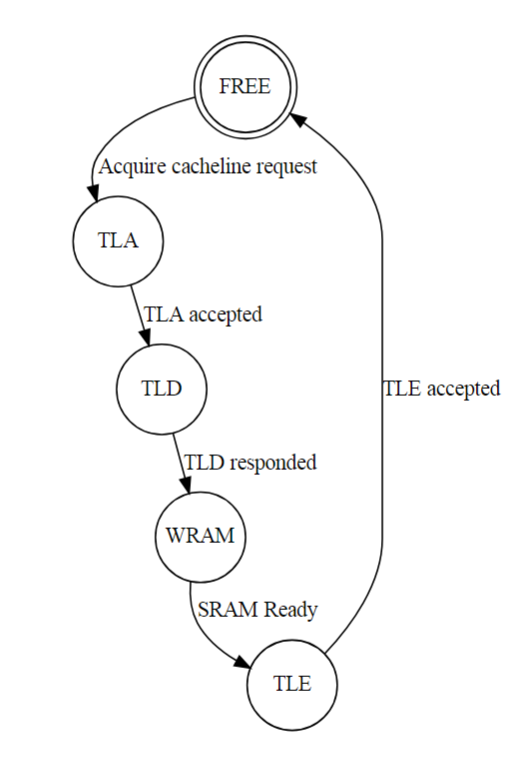
\includegraphics[width=0.5\linewidth]{assets/05/acqfsm.png}
  \caption{权限请求状态机}
  \label{fig:05-acqfsm}
\end{figure}
